% !TEX program = lualatex
% !TEX spellcheck = it_IT
% !TEX root = ../tlinstall.tex

\section*{Prerequisiti (per principianti)}

\begin{figure}
\centering
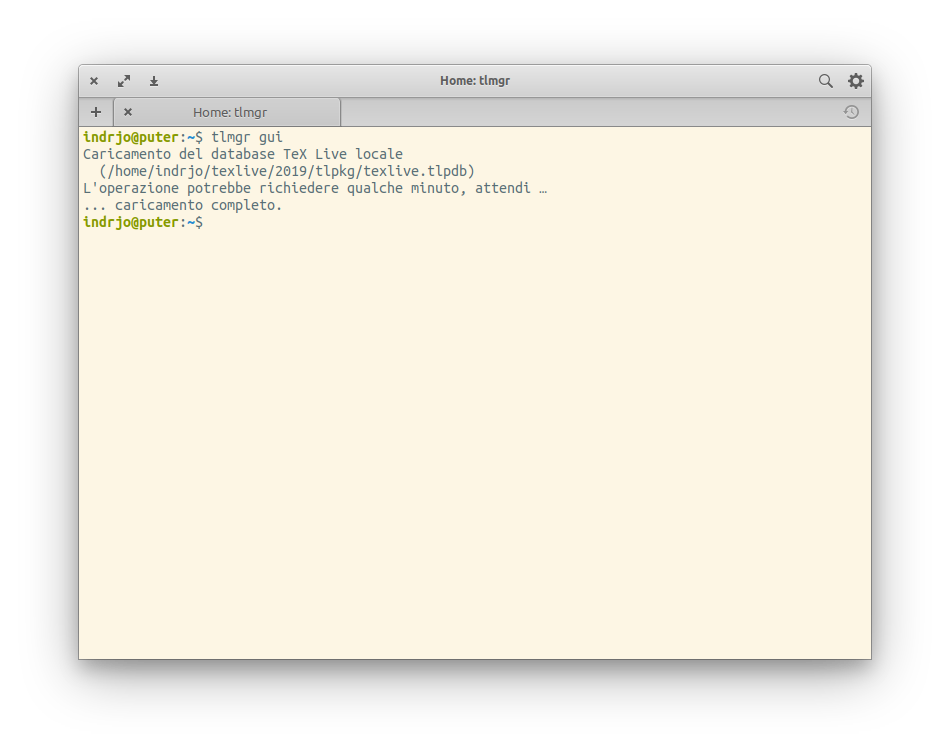
\includegraphics[width=.7\textwidth]{terminale}
\caption{Un esempio di finestra di terminale. (Screenshot da {\sf elementaryOS}).}
\label{fig:terminale}
\end{figure}

Si può essere nuovi al mondo \gnulinux{} o impacciati col computer in generale, ma questa cosa è davvero alla portata di tutti: avviare il terminale (un programma che si presenta come in figura~\ref{fig:terminale}) e dare delle istruzioni attraverso la tastiera. Questo programma non è molto elaborato (ma è molto potente, non ti far ingannare): all'avvio si presenta solo la riga
\begin{lstlisting}
?!...!?@?!...!?:?!...!?$
\end{lstlisting}
seguita da un rettangolino lampeggiante (oppure no, dipende\dots{}): significa che il terminale è in ascolto ed è disponibile a ricevere istruzioni. Il tasto \invio{} fa eseguire i comandi che abbiamo scritto.

Per quello che ci serve in seguito, bisogna inoltre procurarsi i permessi di amministrazione, perché in seguito daremo molti comandi del tipo
\begin{lstlisting}
sudo ?!comando!?
\end{lstlisting}
Ogni volta che viene digitato una frase di questo tipo sul terminale e premuto il tasto \invio{}, compare come riga successiva la richiesta di inserire la password di amministrazione
\begin{lstlisting}
[sudo] password di ?!amministratore!?:
\end{lstlisting}
